\documentclass[twoside,openright,numbers,spanish]{ezthesis}
%% # Opciones disponibles para el documento #
%%
%% Las opciones con un (*) son las opciones predeterminadas.

%%
%% Formato de las referencias bibliogr'aficas:
%%   numbers          - numeradas, p.e. [1]
%%   authoryear (*)   - por autor y a'no, p.e. (Newton, 1997)
%%
%% Opciones adicionales:
%%   spanish         - tesis escrita en espa'nol
%%
%% Desactivar opciones especiales:
%%   nobibtoc   - no incluir la bibiolgraf'ia en el 'Indice general
%%   nofancyhdr - no incluir "fancyhdr" para producir los encabezados
%%   nocolors   - no incluir "xcolor" para producir ligas con colores
%%   nographicx - no incluir "graphicx" para insertar gr'aficos
%%   nonatbib   - no incluir "natbib" para administrar la bibliograf'ia

%% Paquetes adicionales requeridos se pueden agregar tambi'en aqu'i.
%% Por ejemplo:
%\usepackage{subfig}
%\usepackage{multirow}
\usepackage[spanish,activeacute]{babel}
\usepackage[utf8]{inputenc}
\usepackage{amsmath}
\usepackage{amsthm}
\usepackage{amssymb}
\usepackage{wrapfig}
\usepackage{minted}
\usemintedstyle{colorful}

%% # Datos del documento #
%% Nota que los acentos se deben escribir: \'a, \'e, \'i, etc.
%% La letra n con tilde es: \~n.

\author{Mar\'ia Fernanda Alcal\'a Durand}
\title{Aprendizaje Reforzado para el Juego de Distribuci\'on de Cerveza}
\degree{Maestra en Ciencia de Datos}
\supervisor{Dr. Adolfo Javier de Un\'anue Tiscare\~no}
\institution{Instituto Tecnol\'ogico Aut\'onomo de M\'exico}
\faculty{Divisi'on de Actuar\'ia, Estad\'istica y Matem\'aticas}
\department{Departamento Acad'emico de Matem\'aticas}

%% # M'argenes del documento #
%% 
%% Quitar el comentario en la siguiente linea para austar los m'argenes del
%% documento. Leer la documentaci'on de "geometry" para m'as informaci'on.

%\geometry{top=40mm,bottom=33mm,inner=40mm,outer=25mm}

%% El siguiente comando agrega ligas activas en el documento para las
%% referencias cruzadas y citas bibliogr'aficas. Tiene que ser *la 'ultima*
%% instrucci'on antes de \begin{document}.
\hyperlinking
\begin{document}

\graphicspath{{figs/}}

%% # Portada de la tesis #
%% ## Construye tu propia portada ##
%% 
%% Una portada se conforma por una secuencia de "Blocks" que incluyen
%% piezas individuales de informaci'on. Un "Block" puede incluir, por
%% ejemplo, el t'itulo del documento, una im'agen (logotipo de la universidad),
%% el nombre del autor, nombre del supervisor, u cualquier otra pieza de
%% informaci'on.
%%
%% Cada "Block" aparece centrado horizontalmente en la p'agina y,
%% verticalmente, todos los "Blocks" se distruyen de manera uniforme 
%% a lo largo de p'agina.
%%
%% Nota tambi'en que, dentro de un mismo "Block" se pueden cortar
%% lineas usando el comando \\
%%
%% El tama'no del texto dentro de un "Block" se puede modificar usando uno de
%% los comandos:
%%   \small      \LARGE
%%   \large      \huge
%%   \Large      \Huge
%%
%% Y el tipo de letra se puede modificar usando:
%%   \bfseries - negritas
%%   \itshape  - it'alicas
%%   \scshape  - small caps
%%   \slshape  - slanted
%%   \sffamily - sans serif
%%
%% Para producir plantillas generales, la informaci'on que ha sido inclu'ida
%% en el archivo principal "tesis.tex" se puede accesar aqu'i usando:
%%   \insertauthor
%%   \inserttitle
%%   \insertsupervisor
%%   \insertinstitution
%%   \insertdegree
%%   \insertfaculty
%%   \insertdepartment
%%   \insertsubmitdate
%\maketitle

\begin{titlepage}
\begin{center}
\Large {INSTITUTO TECNOLÓGICO AUTÓNOMO DE MÉXICO}

 \vspace{0.5 cm}
  \centering
    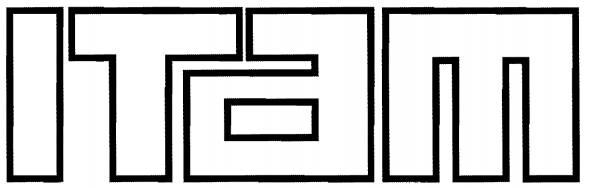
\includegraphics[scale=0.5]{logoITAM.jpg}

 \vspace{0.5 cm}
 \textbf{Aprendizaje Reforzado para el Juego de la Distribuci\'on de Cerveza}
  \vspace{2 cm}\\
  \Huge{\textbf{T \ \ \ \ \ \ E \ \ \ \ \ S \ \ \ \ \ I \ \ \ \ \ \ S}}
    \vspace{.4cm}\\
  \Large{QUE  \ \ PARA \ \ \ OBTENER \ \ \ EL \ \ \ TÍTULO \ \ DE 
   \vspace{.4cm}\\
  MAESTRA EN CIENCIA DE DATOS 
   \vspace{.4cm}\\
  P \ \ \ \ \ \ \ R \ \ \ \ \ \ E \ \ \ \ \ \ S \ \ \ \ \ \ E \ \ \ \ \ \ N \ \ \ \ \ \ T \ \ \ \ \ \ \ A 
   \vspace{.4cm}\\
 \textbf{MAR\'IA \ \ FERNANDA\ \ ALCAL\'A \ \ DURAND}}
    \vspace{1 cm}\\
\normalsize \textbf{ASESOR: DR. ADOLFO JAVIER DE UN\'ANUE TISCARE\~NO}
\vspace{1cm}\\
MÉXICO, D.F \hfill{2018}
\end{center}
\end{titlepage}

%% Nota 1:
%% Se puede agregar un escudo o logotipo en un "Block" como:
%%   \TitleBlock{\includegraphics[height=4cm]{escudo_uni}}
%% y teniendo un archivo "escudo_uni.pdf", "escudo_uni.png" o "escudo_uni.jpg"
%% en alg'un lugar donde LaTeX lo pueda encontrar.

%% Nota 2:
%% Normalmente, el espacio entre "Blocks" se extiende de modo que el
%% contenido se reparte uniformemente sobre toda la p'agina. Este
%% comportamiento se puede modificar para mantener fijo, por ejemplo, el
%% espacio entre un par de "Blocks". Escribiendo:
%%   \TitleBlock{Bloque 1}
%%   \TitleBlock[\bigskip]{Bloque2}
%% se deja un espacio "grande" y de tama~no fijo entre el bloque 1 y 2.
%% Adem'as de \bigskip est'an tambi'en \smallskip y \medskip. Si necesitas
%% aun m'as control puedes usar tambi'en, por ejemplo, \vspace*{2cm}.




%% # Prefacios #
\preface
%% Las secciones del "prefacio" inician con el comando \prefacesection{T'itulo}
%% Este tipo de secciones *no* van numeradas, pero s'i aparecen en el 'indice.
%%
%% Si quieres agregar una secci'on que no vaya n'umerada y que *tampoco*
%% aparezca en el 'indice, usa entonces el comando \chapter*{T'itulo}
%%

\newpage
\mbox{}
\thispagestyle{empty} % para que no se numere esta página

\newpage
\thispagestyle{empty}
Con fundamento en los art'iculos 21 y 27 de la Ley Federal del
Derecho de Autor y como titular de los derechos moral y patrimonial de la obra titulada ``\textbf{Aprendizaje Reforzado para el Juego de Distribuci\'on de Cerveza}'', otorgo de manera gratuita y permanente al Instituto Tecnol'ogico Aut'onomo de M'exico y a la Biblioteca Ra'ul Baill\`eres Jr., autorizaci'on para que fijen la obra en cualquier medio, incluido el electr'onico, y la divulguen entre sus usuarios, profesores, estudiantes o terceras personas, sin que pueda percibir por tal divulgación una contraprestación.

\vspace{20 mm}
\begin{center}
Mar'ia Fernanda Alcal'a Durand\\

\vspace{20 mm}
\makebox[2in]{\hrulefill}\\
FECHA\\
\vspace{20 mm}
\makebox[2in]{\hrulefill}\\
FIRMA
\end{center}

\newpage
\mbox{}
\thispagestyle{empty} % para que no se numere esta página


\prefacesection{Agradecimientos}

Evidentemente esta no es la forma final. Pero a grandes rasgos, \\

Mi mam\'a, mi novio, mi familia y mi asesor.\\

Amigos que me han ayudado sustancialmente: Paris M\'endez, Jan Vlachy, Felipe Gerard, Laila Wahedi.

\newpage
\mbox{}
\thispagestyle{empty} % para que no se numere esta página

\prefacesection{Resumen}

Este trabajo de Tesis propone representar el conocido \textit{Juego de la Distribuci\'on de Cerveza} como un modelo multiagente de cadena de suministro, a\~nadiendo una restricci\'on tal que se aproxime m\'as a un problema del mundo real: la producci\'on de materia prima es finita y solamente ocurre en un periodo espec\'ifico. El acercamiento elegido es la aplicaci\'on de dos m\'etodos de aprendizaje reforzado: \textit{Policy Iteration} y \textit{Q-learning}; ambas t\'ecnicas encuentran estrategias aplicables para todos los agentes. Se demuestra que con \textit{Policy Iteration} se encuentra un conjunto de pol\'iticas que les reportan mayores utilidades que algunas estrategias b\'asicas, bajo un esquema de recompensas y castigos. Por otro lado, \textit{Q-learning} demuestra ser un algoritmo pesado computacionalmente y, aunque proporciona estrategias para los agentes, no puede responder a cambios tan r\'apidamente como \textit{Policy Iteration}.\\

Se concluye que el aprendizaje reforzado no solamente es eficiente, sino suficientemente flexible como para identificar cambios permanentes en la demanda y adaptar las consecuentes pol\'iticas de compra. Asimismo, se muestra evidencia de que para cada agente en la cadena, es preferible seguir estrategias optimizadas independientemente de las decisiones de los dem\'as agentes. Finalmente, se explora la posibilidad de que en subsecuentes trabajos, se a\~nadan estrategias diferentes o restricciones adicionales al \textit{Problema de la Distribuci\'on de la Cerveza} para obtener modelos m\'as fieles a las condiciones del mundo externo y, por lo tanto, utilizables en un contexto real.\\

\textbf{T\'erminos clave}
Juego de la Distribuci\'on de Cerveza, Aprendizaje Reforzado, Iteraci\'on de Pol'itica, Q-aprendizaje


%% # 'Indices y listas de contenido #
%% Quitar los comentarios en las lineas siguientes para obtener listas de
%% figuras y cuadros/tablas.
\tableofcontents
%\listoffigures
%\listoftables

%% # Cap'itulos #
\cuerpo
\chapter{Introducci'on}

\textit{Necesito una cita cool para empezar mi tesis.}
\begin{flushright}
 Fleo
 \end{flushright}

\vspace{10 pt}


%business dynamics
%sistemas complejos adaptativos
%poner ejemplos?

%dynamic stability : edge of chaos. no es que sean caóticos sino que la mayor parte de las fluctuaciones pequeñas se las comen los feedback, pero la línea de qué es "pequeño" no es nada clara
%ley de Ashby: para poder controlar algo, se necesita al menos igual nivel de complejidad


Uno de las principales dificultades de las cadenas de suministro es que los agentes encargados de optimizar las estrategias solamente pueden tomar decisiones "dentro" del eslabón en el que se encuentran, y no tienen información más allá de los eslabones inmediatamente conectados. Así, la información acerca de la demanda del consumidor se va diluyendo en cada nivel, además de que las decisiones tomadas tienen repercusiones más allá del futuro inmediato. \\

Los agentes optimizadores deben tratar de inferir el patrón global por medio de información local bastante restringida. Sin embargo, los datos que reciben obedecen al tiempo real y no tienen la oportunidad de repetir experimentos.\\

Un modelo computacional que se comporte suficientemente parecido al mundo real, en el que todos los demás eslabones tomen estrategias que también maximizarían sus beneficios podría dar una opción: el experimento es replicable tantas veces como sea necesario y cada eslabón puede conocer una estrategia óptima para una gran cantidad de demandas de consumidor posibles.\\

En este trabajo se modelará el Problema de Distribución de Cerveza, \textit{The Beer Distribution Game}, planteado por primera vez por el profesor \citet{Forrester}, en la Escuela de Administraci\'on y Direcci\'on de Empresas Sloan del MIT en los años 60, para ilustrar el concepto de \textit{efecto l\'atigo}. \\


\chapter{El Problema: Juego de Distribuci\'on de la Cerveza}

El \textit{Juego de la Distribución de Cerveza} ejemplifica la relaci\'on causal entre la toma de decisiones de cada agente (que no tiene informaci\'on global) con el comportamiento de todo el sistema, en este caso una cadena de suministro. Asimismo, a falta de una estrategia \'optima, inherentemente presenta el efecto l\'atigo: el retraso en la informaci\'on entre agentes causa que, a trav\'es del tiempo, el comportamiento de cada uno se vuelva menos constante cuanto m\'as lejos se encuentre del consumidor final. Por \'ultimo, evidencia las ineficiencias inherentes a tratar de resolver el problema enfoc\'andose en los agentes, ignorando que es un sistema completo. 

%business dynamics
%sistemas complejos adaptativos
%poner ejemplos?

%dynamic stability : edge of chaos. no es que sean caóticos sino que la mayor parte de las fluctuaciones pequeñas se las comen los feedback, pero la línea de qué es "pequeño" no es nada clara
%ley de Ashby: para poder controlar algo, se necesita al menos igual nivel de complejidad


\section{Cadenas de Suministro}

Para plantear correctamente el \textit{Problema de la Distribuci\'n de Cerveza}, es necesario entender el concepto de una cadena de suministro. \\

Para construir sobre la definici\'on de \citet{Sterman} descrita en el cap\'itulo anterior, una cadena de suministro (en ingl\'es, \textit{supply chain}), seg\'un \citet{Jacobs}, es un proceso que desplaza informaci\'on y material con destino y origen en los procesos de manufactura y servicio de la empresa. Una manera com\'un de representar el comportamiento de una cadena como un modelo es a trav\'es de existencias, flujos, ciclos y agentes\footnote{Existen muchas otras maneras, como las redes de Petri, ampliamente utilizadas en la teor\'ia de aut\'omatas. ( \citet{Shiflet})}. Por ejemplo, en una simplificaci\o'n de producci\'on automotriz que se puede observar en la figura \ref{automotriz}, se puede observar un ejemplo en el cual se representa cada eslab\'on como un agente (la f\'abrica de partes, la ensambladora, el taller de pintura y la agencia de venta), los flujos de producto como las entradas y salidas de materia en cada eslab\'on (por ejemplo, la f\'abrica de partes tiene como insumos metal y pl\'astico, mientras que el taller de pintura tiene como insumo el auto ensamblado y litros de pintura), los flujos de informaci\'on se suponen globales y sin retraso, y los ciclos pueden depender de estacionalidad, disponibilidad o simple predisposici\'on.\\

\begin{figure}[ht]
\caption{\textit{Ejemplo de simplificaci\'on de una cadena de suministro automotriz}}
\label{automotriz}
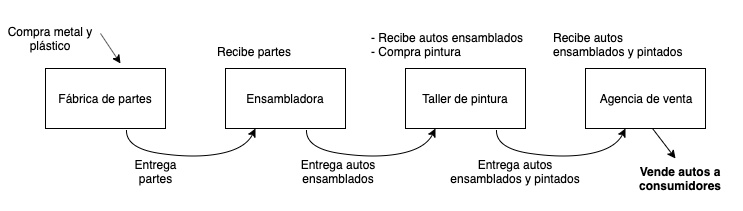
\includegraphics[width=15cm]{tesis_tex/figs/auto_chain_simple.png}
\centering
\end{figure}


El estudio de las cadenas de suministro puede cubrir un campo vasto, dado que existen una gran cantidad de problemas relacionados a ellas: transporte, log\'istica, manejo de inventario, optimizaci\'on de la localizaci\'on geogr\'afica para cada uno de los eslabones, sustentabilidad, etc. Sin embargo, una vez que la cadena est\'a en funcionamiento, uno de las principales dificultades es que los agentes encargados de optimizar las estrategias de demanda y producci\'on de cada eslab\'on solamente pueden tomar decisiones ``dentro'' de aquel en el que se encuentran, y no tienen informaci\'on m\'as all\'a de los eslabones inmediatamente conectados, solamente una estimaci\'on (en ingl\'es \textit{forecast}) que representa su mejor predicci\'on de tal comportamiento. As\'i, la informaci\'on acerca de la demanda del consumidor se va diluyendo en cada nivel, además de que las decisiones tomadas tienen repercusiones m\'as all\'a del futuro inmediato. \\

El objetivo principal de cada agente es minimizar los costos al tiempo de maximizar los ingresos, donde los costos pueden no ser flujos de dinero sino, por ejemplo, castigos por \'ordenes no cumplidas o varianza alta en la producci\'on que implique mayores costos de mantenimiento. Para llegar a este objetivo, cada uno de ellos debe tratar de inferir el patr\'on de demanda del consumidor, que llegar\'a distorsionado a \'el, por medio de información local bastante restringida. Al tener una estimaci\'on \'util de tal patr\'on, as\'i como del comportamiento de sus eslabones inmediatamente conectado, puede crear su estrategia de inventario y producci\'on para maximizar su utlidad. Volviendo al ejemplo anterior de la producci\'on automotriz, la f\'abrica de partes debe ordenar metal y pl\'astico suficiente para producir y cubrir la demanda de la planta ensambladora, pero ambos eslabones deben producir manteniendo en mente que la tendencia de demanda proviene, al final, del consumidor. Sin embargo, la planta no tiene ning\'un incentivo real para compartir con la f\'abrica la cantidad exacta de autos ensamblados que produce o que vende cada periodo al taller de pintura. Esto obliga a cada eslab\'on a contar solamente con datos limitados, adem\'as de que los datos de demanda que reciben obedecen al tiempo real y los agentes no tienen la oportunidad de repetir experimentos.\\

Un modelo computacional que se comporte suficientemente parecido al mundo real, en el que todos los demás eslabones tomen estrategias que también maximizarían sus beneficios podría dar una opción: el experimento es replicable tantas veces como sea necesario y cada eslabón puede conocer una estrategia óptima para una gran cantidad de demandas de consumidor posibles.\\

\section{El Juego de la Distribuci\'on de Cerveza}

El Juego de la Distribuci\'on de Cerveza (en ingl\'es \textit{The Beer Distribution Game}) \cite{StermanArt} fue planteado por primera vez en la Escuela de Administraci\'on y Direcci\'on de Empresas Sloan del MIT para ejemplificar el \textit{efecto l\'atigo}, llamado as\'i por la similaridad que tiene el comportamiento la informaci\'on en cada nivel de la cadena con el patr\'on ondulado que toma un l\'atigo, en el cual existe una mayor amplitud de onda (comparable con el ruido o la varianza en la informaci\'on) al alejarse del punto de origen (comparable al consumidor). \\

En su forma de juego de mesa, se presenta com\'unmente a alumnos reci\'en ingresados a distintas escuelas de negocios. El MIT (\citet{Dizikes}) y varios autores como \citet{Sterman} han publicado que, independientemente del rol que jueguen y de cu\'anta experiencia y preparaci\'on en negocios tengan, los humanos consistentemente fallan en encontrar la estrategia para maximizar la utilidad. Para nosotros los humanos, es sumamente dif\'icil pensar de manera no lineal y tomar en cuenta efectos como retrasos (tanto en entrega de los pedidos como en la informaci\'on) o la retroalimentaci\'on en los ciclos (cuando hay inventario sobrante, puede ser llevado al siguiente periodo). Estos conceptos son manejados correctamente cuando se modelan como efectos de sistemas din\'amicos, tarea considerablemente m\'as f\'acil para una computadora que para una persona. Asimismo, nota que es inevitable la frustraci\'on, y que incluso los equipos que obtienen los mejores resultados del juego terminan lejos del \'optimo te\'orico.\\

\section{Principales caracter\'isticas}

El juego consiste, a grandes rasgos, en asignar a cada agente un rol en una cadena de suministro de cerveza, buscando maximizar las ganancias individuales al final del juego.\\

Existen cuatro jugadores: minorista (\textit{retail}), mayorista (\textit{wholesale}), distribuidor (\textit{regional warehouse}) y f\'abrica (\textit{factory}). Dentro del juego transcurren 52 semanas (un a\~no), durante las cuales existe una demanda del consumidor, que se revela al inicio de la semana. De esta manera, el minorista debe cubrir (restringido a su inventario) la demanda del consumidor, y decidir la orden que pedir\'a al mayorista para recibir la siguiente semana. Cada jugador sigue instrucciones similares, con el objetivo de maximizar sus ganancias al final del juego.\\

Todos los agentes cuentan con un inventario inicial de cajas de cerveza, y deben manejar correctamente su inventario para poder cumplir con la demanda del agente siguiente, al tiempo de minimizar los costos de almacenamiento por cada caja. Todos reciben ingresos por vender cajas de cerveza, e incurren en costos por comprar inventario, almacenar inventario, y por \'ultimo, una penalizaci\'on por no cubrir las \'ordenes. La estructura del juego se puede observar en la figura \ref{structure}.\\


\begin{figure}[ht]
\label{structure}
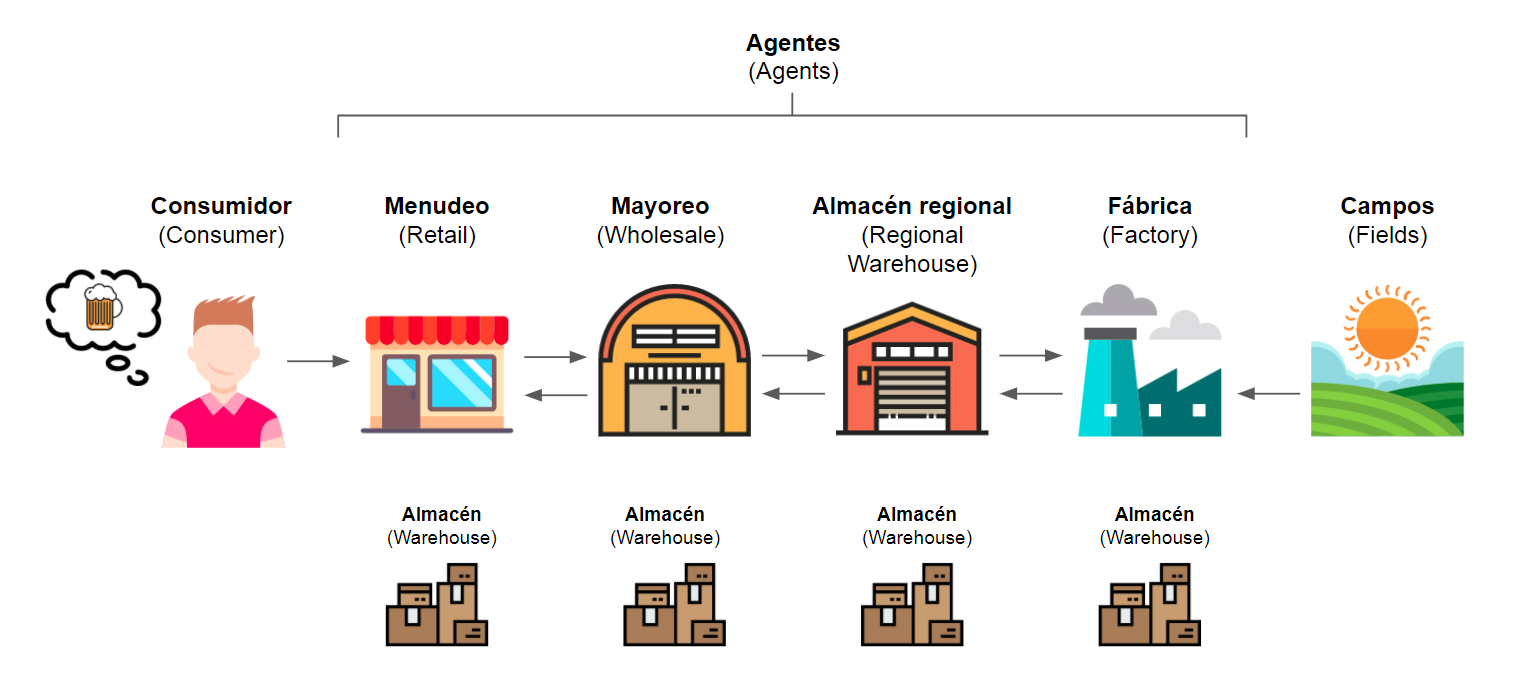
\includegraphics[width=15cm]{tesis_tex/figs/beer_distribution_game_structure.PNG}
\caption[Estructura del Juego de Distribución de Cerveza]{Estructura del Juego de Distribución de Cerveza\protect\footnotemark}
\centering
\end{figure}

\footnotetext{Iconos creados por Freepik, Iconnice, Roundicons en \textit{www.flaticon.com}}

De manera general, las variables que tienen efecto en la soluci\'on de este problema son:

\begin{itemize}
    \item Demanda del consumidor durante el a\~no
    \item Producci\'on (oferta) de los campos durante el a\~no
    \item Precio de la cerveza (se supone el mismo margen nominal para cada agente)
    \item Costo de almacenaje (se supone igual para todos los agentes)
    \item Costo de oportunidad por \'ordenes no cumplidas (se supone igual para todos los agentes)
    \item Inventario inicial (puede variar por agente)
\end{itemize}

Sin embargo, en cada tiempo $t$, cada agente se enfrenta a factores espec\'ificos que afectan su decisi\'on de compra para el siguiente d\'ia, cuyo diagrama se puede consultar en la figura \ref{causal}. Este conjunto de factores ha sido mapeado anteriormente por \citet{Duggan} y \citet{Grasl}, desde el punto de vista de diagramas causales. Una gran parte de la complejidad de este problema se puede identificar aqu\'i: ning\'un agente tienen visibilidad del proceso an\'alogo para su agente superior, por lo tanto debe actuar bajo informaci\'on incompleta y con indicaciones de comportamiento, tales como evitar el costo por \'ordenes no cumplidas y reaccionar a los cambios en la demanda del agente inferior.

\begin{figure}[ht]
\caption{Diagrama Causal para un agente del Juego}
\label{causal}
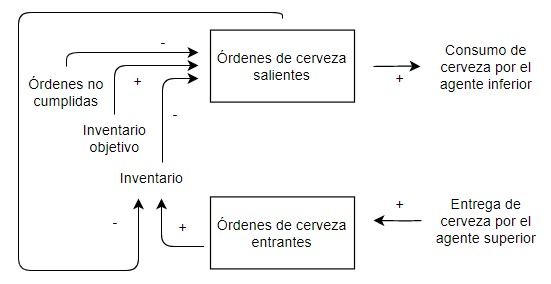
\includegraphics[width=10cm]{tesis_tex/figs/beer_distribution_game_causal.PNG}
\centering
\end{figure}

Este diagrama causal describe un diagrama de existencias y flujos (\textit{stock and flow diagram}), el cual describe las ecuaciones del sistema que ser\'an presentadas en las secciones siguientes. Se puede consultar en la figura \ref{stockflow}

\begin{figure}[ht]
\caption{Diagrama de Existencias y Flujos para el Juego}
\label{stockflow}
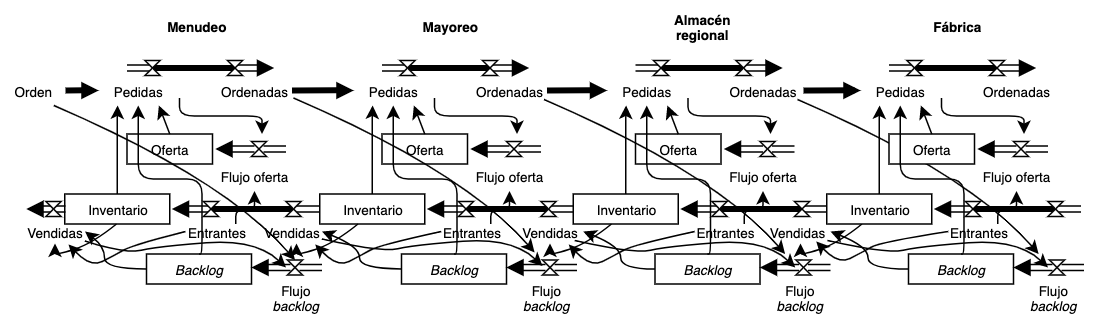
\includegraphics[width=14cm]{tesis_tex/figs/beer_distribution_game_stock_flow.PNG}
\centering
\end{figure}

Todas las variables, menos la demanda del consumidor y la producci\'on en los campos, pueden ser declaradas para el sistema (igual para todos los agentes) o individualmente (diferente para cada agente). Como se ver\'a m\'as adelante, el sistema es sumamente sensible a peque\~nos cambios en cualquiera de las variables; por ejemplo, si un agente comienza el juego con suficiente inventario para todo el a\~no, el agente superior nunca podr\'a venderle cerveza e incurrir\'a solamente en costos por almacenaje.

\subsection{El Efecto Látigo}

El \textit{Efecto Látigo} es un fen\'omeno que se produce en cadenas de suministro. Se llama de esa manera porque, mientras m\'as ``arriba'' en la cadena de suministro se encuentre un agente (es decir, m\'as lejos del contacto directo con el comprador), m\'as distorsionada es la informaci\'on que tiene acerca de la verdadera demanda del comprador; tal varianza se puede visualizar como una curva que asemeja un l\'atigo. \citet{Chaharsooghi} nota que la distorsi\'on se debe mayormente a tres factores: prejuicios en la informaci\'on de la demanda por parte de los miembros cercanos al consumidor, retraso en el intercambio de informaci\'on entre los miembros de la cadena y soporte log\'istico inapropiado a trav\'es de la cadena. \\

El caso m\'as com\'un de efecto l\'atigo surge por la necesidad de un inventario de seguridad, para asegurar que un agente no incurrir\'a en costos por \'ordenes no cumplidas. Cada agente a\~nadir\'ia cantidad a su orden, causando una orden artificialmente inflada para el agente m\'as lejano al consumidor. Si el comportamiento del consumidor no cambia, las \'ordenes se estabilizar\'ian en un nivel inferior despu\'es de un tiempo, pero los agentes superiores podr\'ian estar incurriendo en un mayor costo de almacenamiento en el mismo tiempo. Adem\'as, tener menos claridad acerca de la demanda real del consumidor \\

El efecto puede ejemplificar con el siguiente escenario:

\begin{enumerate}
    \item El consumidor, que generalmente compra $6$ cervezas, ahora quiere $10$, pero la tienda minorista solamente cuenta con $7$. El minorista le venderá todo su inventario, pues es la acci\'on que maximiza su ganancia. Despu\'es, debe decidir si volverá a tener un inventario de $6$ o si debe pedir un número mayor de cervezas, atendiendo la posible creciente demanda. Decide pedir $9$ cervezas al siguiente nivel, la tienda de mayoreo.
    \item El mayorista cuenta con $17$ cervezas. Llena el pedido del minorista, pero decide que ten\'ia guardado demasiado inventario, as\'i que se queda con $8$ cervezas en su almac\'en, sin hacer una orden al siguiente nivel, la tienda de distribución.
    \item La tienda de distribuci\'on decide no comprar unidades a la f\'abrica, dado que no disminuy\'o su inventario.
    \item La f\'abrica conoce la restricci\'on de estacionalidad de la cebada, as\'i que compra una m\'inima cantidad a los campos.
\end{enumerate}

En este escenario, el mayorista obtuvo informaci\'on distorsionada acerca del repentino crecimiento en la demanda del comprador, mientras que la tienda de distribución podr\'ia incluso interpretar que el comprador disminuy\'o su consumo. Si este comportamiento se mantiene durante algunos periodos m\'as, recibir\'ia la noticia (por medio de un incremento en las \'ordenes regulares) con un retraso considerable, lo cual inevitablemente causar\'a perturbaciones en sentido contrario cuando incrementen sus \'ordenes recibidas.\\

En el caso de que la demanda sea determinista (con un castigo por \'ordenes no cumplidas), la orden \'optima en cada tiempo para cada miembro de la cadena es ``una por una'', es decir, demandar al agente superior exactamente lo mismo que fue demandado por el agente inferior.

\subsection{La din\'amica de las existencias y flujos}

Las existencias y flujos (\textit{stocks and flows}) son componentes b\'asicos en un sistema din\'amico \footnote{Para mayor profundidad acerca de sistemas din\'amicos y el comportamiento de las existencias y flujos, \citet{Sterman} profundiza y provee de las bases adecuadas para sistemas m\'as complejos.}. Las existencias son acumulaciones basadas en la diferencia entre los flujos entrantes y los salientes. El flujo neto a una existencia en un tiempo determinado $t$ es la tasa de cambio de la existencia en el tiempo $t$:

$$
Existencia(t) = \int_{t_{0}}^t [Entrada(s) - Salida(s)]ds + Existencia(t_{0}) 
$$

Es com\'un que en un sistema con varias existencias con sus respectivos flujos ocurran retrasos. Esto sucede porque, en general, los flujos de entrada y salida son gobernados por decisiones diferentes. En el Juego de Distribuci\'on de Cerveza, para cada agente, su flujo de salida depende de la demanda del agente inmediatamente inferior limitada por su propia existencia, y su flujo de entrada depende de su propia demanda limitada por la existencia del agente inmediatamente superior. Esto, aunado a un comportamiento ligeramente aleatorio de la demanda del consumidor, puede desembocar en insuficiencia de existencias para cualquier agente en cualquier tiempo $t$. \\

Un sistema est\'a en equilibrio cuando ninguna de sus existencias cambia. Esta condici\'on se obtiene cuando el cambio neto de sus flujos es cero, es decir, cuando el flujo entrante es igual al flujo saliente. \\

La soluci\'on trivial para este equilibrio es que todos los flujos sean nulos (\textit{equilibrio est\'atico}), sin embargo, en el caso de la cadena de suministro, este escenario llevar\'ia a que ning\'un agente tuviera ventas, y por consiguiente, tampoco tuviera ganancias. Una situaci\'on m\'as adecuada ser\'ia un \textit{equilibrio din\'amico}, en el cual las existencias totales se mantienen constantes, pero los flujos son diferences de cero. Para la cerveza, esto significar\'ia que la cantidad de cerveza en los almacenes se mantiene constante, pero cada caja de cerveza se mueve de un agente a otro en alg\'un punto en el tiempo. Sin restricciones de oferta, la situaci\'on ideal tender\'ia a no guardar cerveza en los almacenes. Sin embargo, el efecto l\'atigo, causado por cambios en la demanda del consumidor, complica la estimaci\'on de los flujos entrantes y salientes en cada tiempo, pues para cada agente son desconocidas tanto la demanda del agente inferior como la capacidad del agente superior de cubrir la demanda propia. Existe una complicaci\'on extra al a\~nadir estacionalidad en la producci\'on de los campos de cebada. \\

\section{Acercamiento en el Presente Trabajo}

En este trabajo se modelará el Problema de Distribución de Cerveza, \textit{The Beer Distribution Game}, ampliamente utilizado y explicado por el Profesor \citet{Sterman} en la Escuela de Administraci\'on y Direcci\'on de Empresas Sloan del MIT, como una cadena de suministro, para ilustrar el concepto de \textit{efecto l\'atigo} (en ingl\'es, \textit{bullwhip effect}. Este efecto recibi\'o tal nombre debido a que la varianza en la informaci\'on acerca de la demanda real tiene el mismo comportamiento que un l\'atigo: mientras m\'as lejano se encuentra del origen (consumidor), mayor amplitud tiene la onda (varianza).\\

Existen acercamientos anteriores a este problema, en espec\'ifico \citet{Chaharsooghi} propone ya un acercamiento con \textit{Q-learning} \footnote{Los nombres de los algoritmos ser\'an representados con it\'alicas en este trabajo.} pero sin restricci\'on de estacionalidad en la materia prima, \citet{Strozzi}, por medio de Algoritmos Genéticos, \citet{Kimbrough} y \citet{Zarandi} proponen h\'ibridos de un algoritmo gen\'etico y aprendizaje reforzado.\\

Por otro lado, algunas l\'ineas de investigaci\'on como \citet{Busoniu} se han concentrado en el aspecto de teor\'ia de juegos que compete a este problema: si en un vendedor de menudeo no tiene existencias, los consumidores podr\'an elegir otro. En este caso, los agentes son construidos como adversarios. Dado que en el modelo que se resuelve en el presente trabajo, el sistema se compone de agentes representativos (i.e.. se resuelve la ecuaci\'on para el agente prototipo llamado `tienda de menudeo', pero tal soluci\'on \'optima podr\'ia ser adoptada por cualquier tienda de menudeo espec\'ifica), es equivalente a tener un solo agente, que por s\'i mismo no puede ser ni adversario ni cooperativo, sino solamente maximiza su propia utilidad, as\'i que no se implementar\'a tal metodolog\'ia.\\

Sin embargo, todos los acercamientos anteriores suponen que los campos pueden adaptarse de inmediato a la demanda de la f\'abrica, de cierta manera tienen "producci\'on infinita". Los aportes de este trabajo son:

\begin{enumerate}
    \item Una tendencia de demanda de consumidor de cerveza m\'as flexible y cercana a la vida real, basada en tendencias catalogadas por una agencia de investigaci\'on de los EUA
    \item La imposici\'on de restricciones estacionales en la producci\'on de cebada, basadas en tendencias catalogadas por el departamento de agricultura de los EUA
\end{enumerate}

Tales supuestos cual deber\'ian alterar el comportamiento de los agentes tal que respondan a la tendencia de demanda de consumidor, y mantengan una existencia positiva en sus almacenes para poder enfrentar tal demanda en periodos de baja producci\'on. Esto deber\'ia verse reflejado en estrategias que sigan la curva de producci'on cuando existe una restricci\'on en los campos, o que se asemejen m\'as  a la curva de demanda del consumidor si tal restricci\'on no existe.\\

En la vida real, los agentes tienen acceso a esta informaci\'on, a sus propios datos internos de ventas de a\~nos pasados, a predicciones del a\~no en curso, etc. El modelo que se construir\'a en este trabajo solamente considera los datos p\'ublicos, el cual ser\'ia el caso para un agente completamente nuevo en el juego, pero es una oportunidad de desarrollo futuro.\\

En este trabajo se presentar\'an diversas simulaciones, las cuales reflejan distintos escenarios tanto de condiciones iniciales, como de comportamiento. Se analizar\'a, por ejemplo, qu\'e pasa si un agente comienza el a\~no con suficiente inventario como para cubrir toda la demanda del agente inferior, si solamente un agente sigue una estrategia \'optima, si los costos de almacenamiento son demasiado altos, entre otros.



\chapter{Acercamientos Previos a la Soluci\'on}

\section{Est\'atica: m\'axima ganancia posible}

El sistema tiene una soluci\'on anal\'itica si no existe una restricci\'on en la oferta (es decir, el campo siempre puede cubrir la demanda de la f\'abrica) y cada agente tiene en el d\'ia $n$ informaci\'on acerca de la demanda del d\'ia $n+1$ de su agente inmediatamente inferior. En este caso, los agentes ni siquiera necesitan usar sus almacenes: sencillamente compran cada d\'ia lo necesario para el d\'ia siguiente. Podemos observar el comportamiento de esta soluci\'on en la figura \ref{analytic_1}.

\begin{figure}[ht!]
\caption{Estrategias aprendidas con informaci\'on perfecta}
\label{analytic_1}
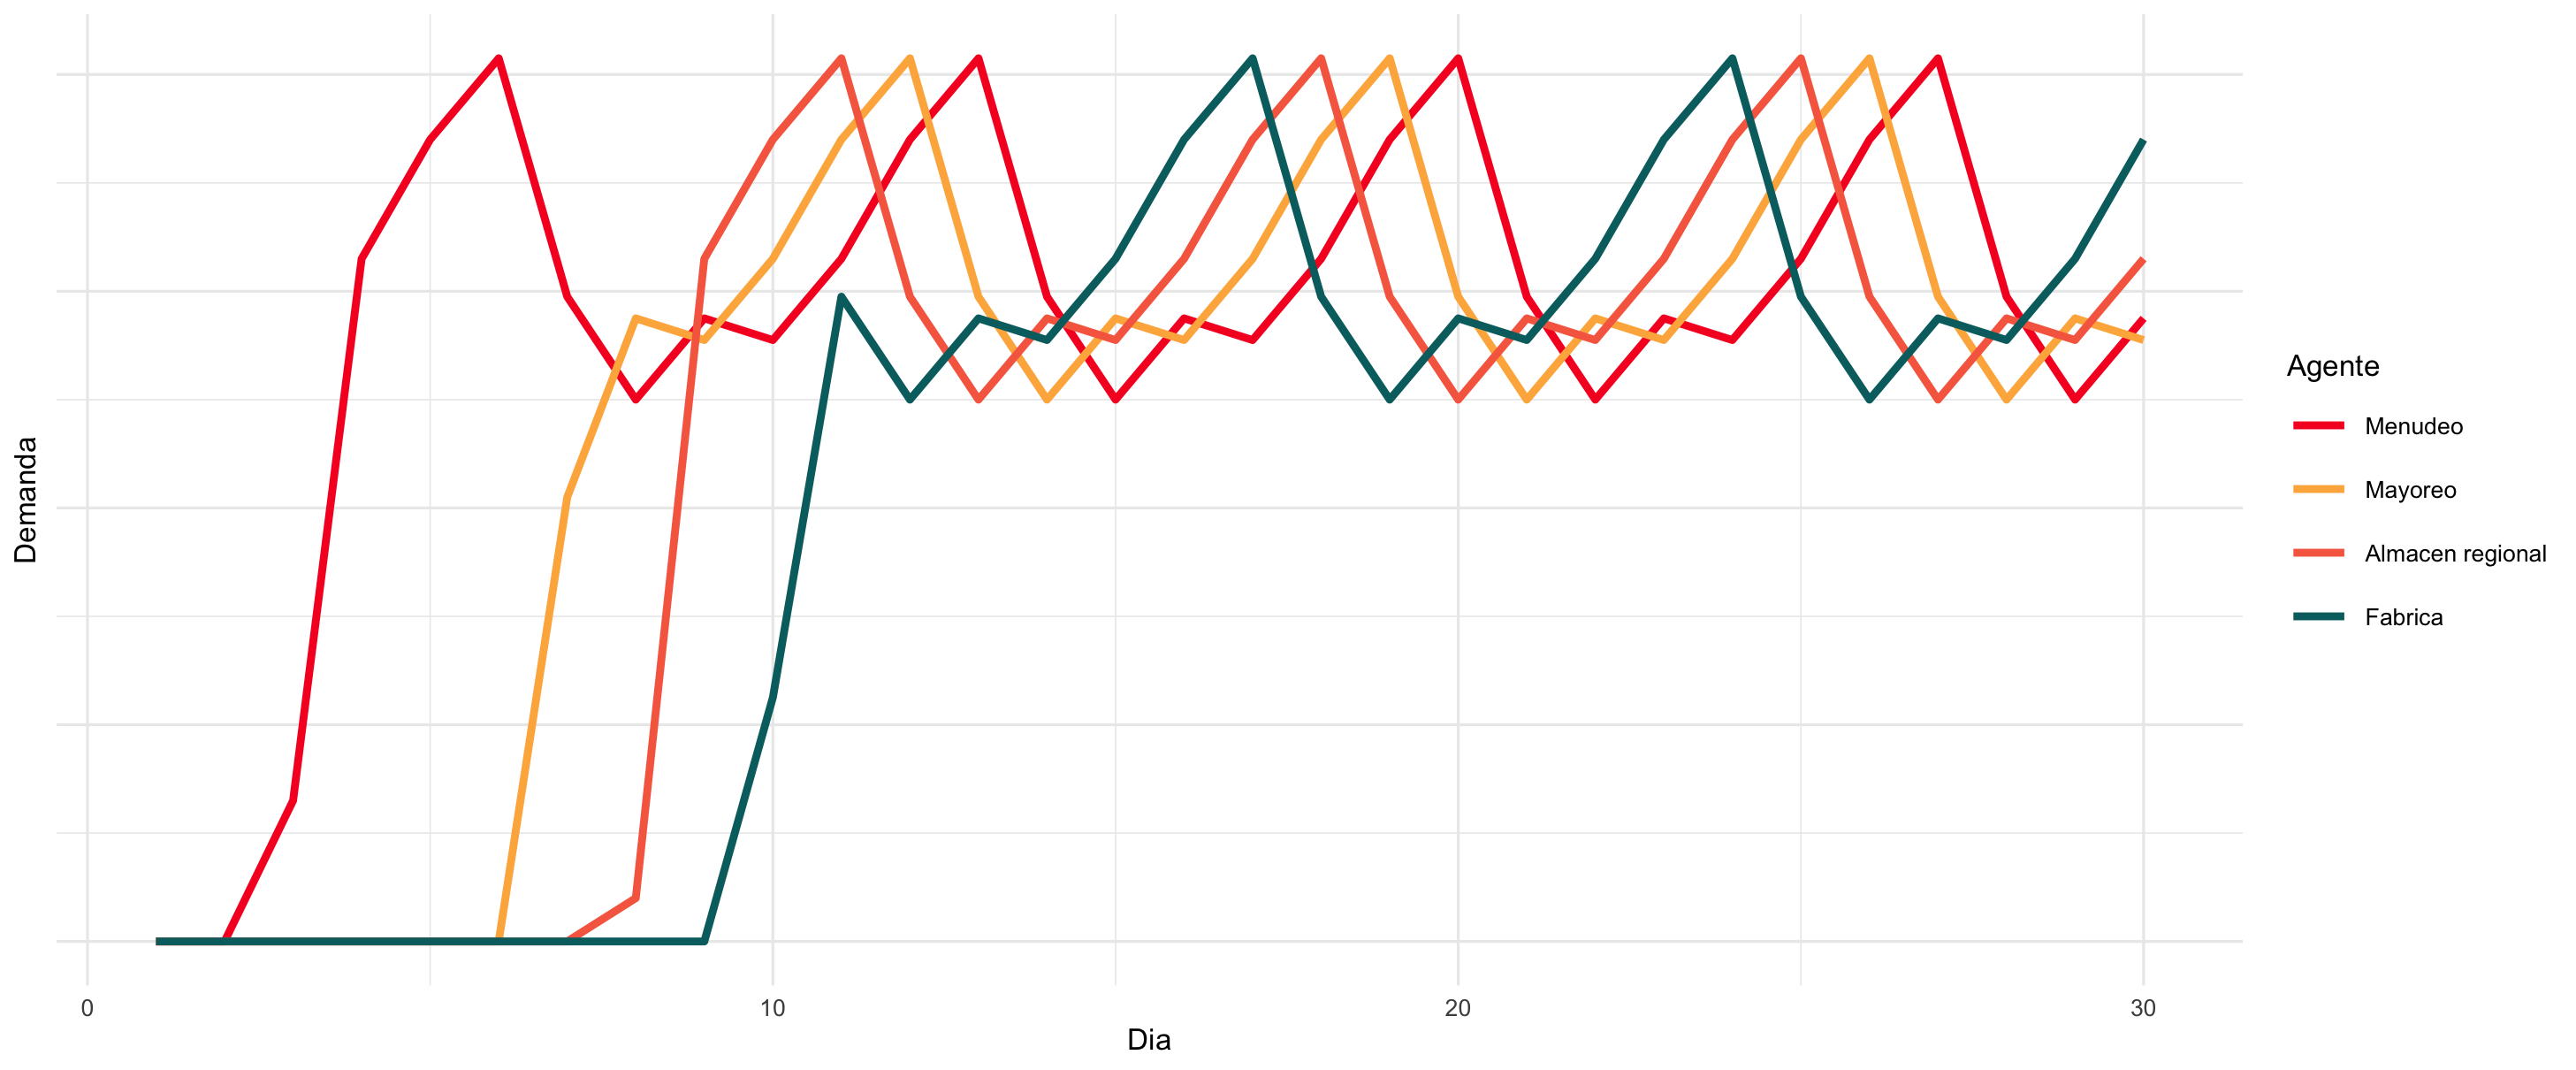
\includegraphics[width=12cm]{tesis_tex/figs/analytic_solution_0_all_0_inv.png}
\centering
\end{figure}

Sin embargo, incluso cuando todos los agentes tienen informaci\'on perfecta, podemos observar una versi\'on muy ligera del efecto l\'atigo. Si el minorista tiene suficiente cerveza para cubrir algunos d\'ias de demanda del consumidor, entonces no tiene incentivo para comprarle al mayorista hasta que su inventario se agote. Esta situaci\'on puede replicarse en los dos niveles superiores, de tal manera que la f\'abrica no recibe nada de informaci\'on acerca de la demanda del consumidor durante una cantidad considerable de tiempo. Este efecto se puede observar en la figura \ref{analytic_2}.

\begin{figure}[ht!]
\caption{Retraso en visibilidad de la informaci\'on para agentes en la cadena}
\label{analytic_2}
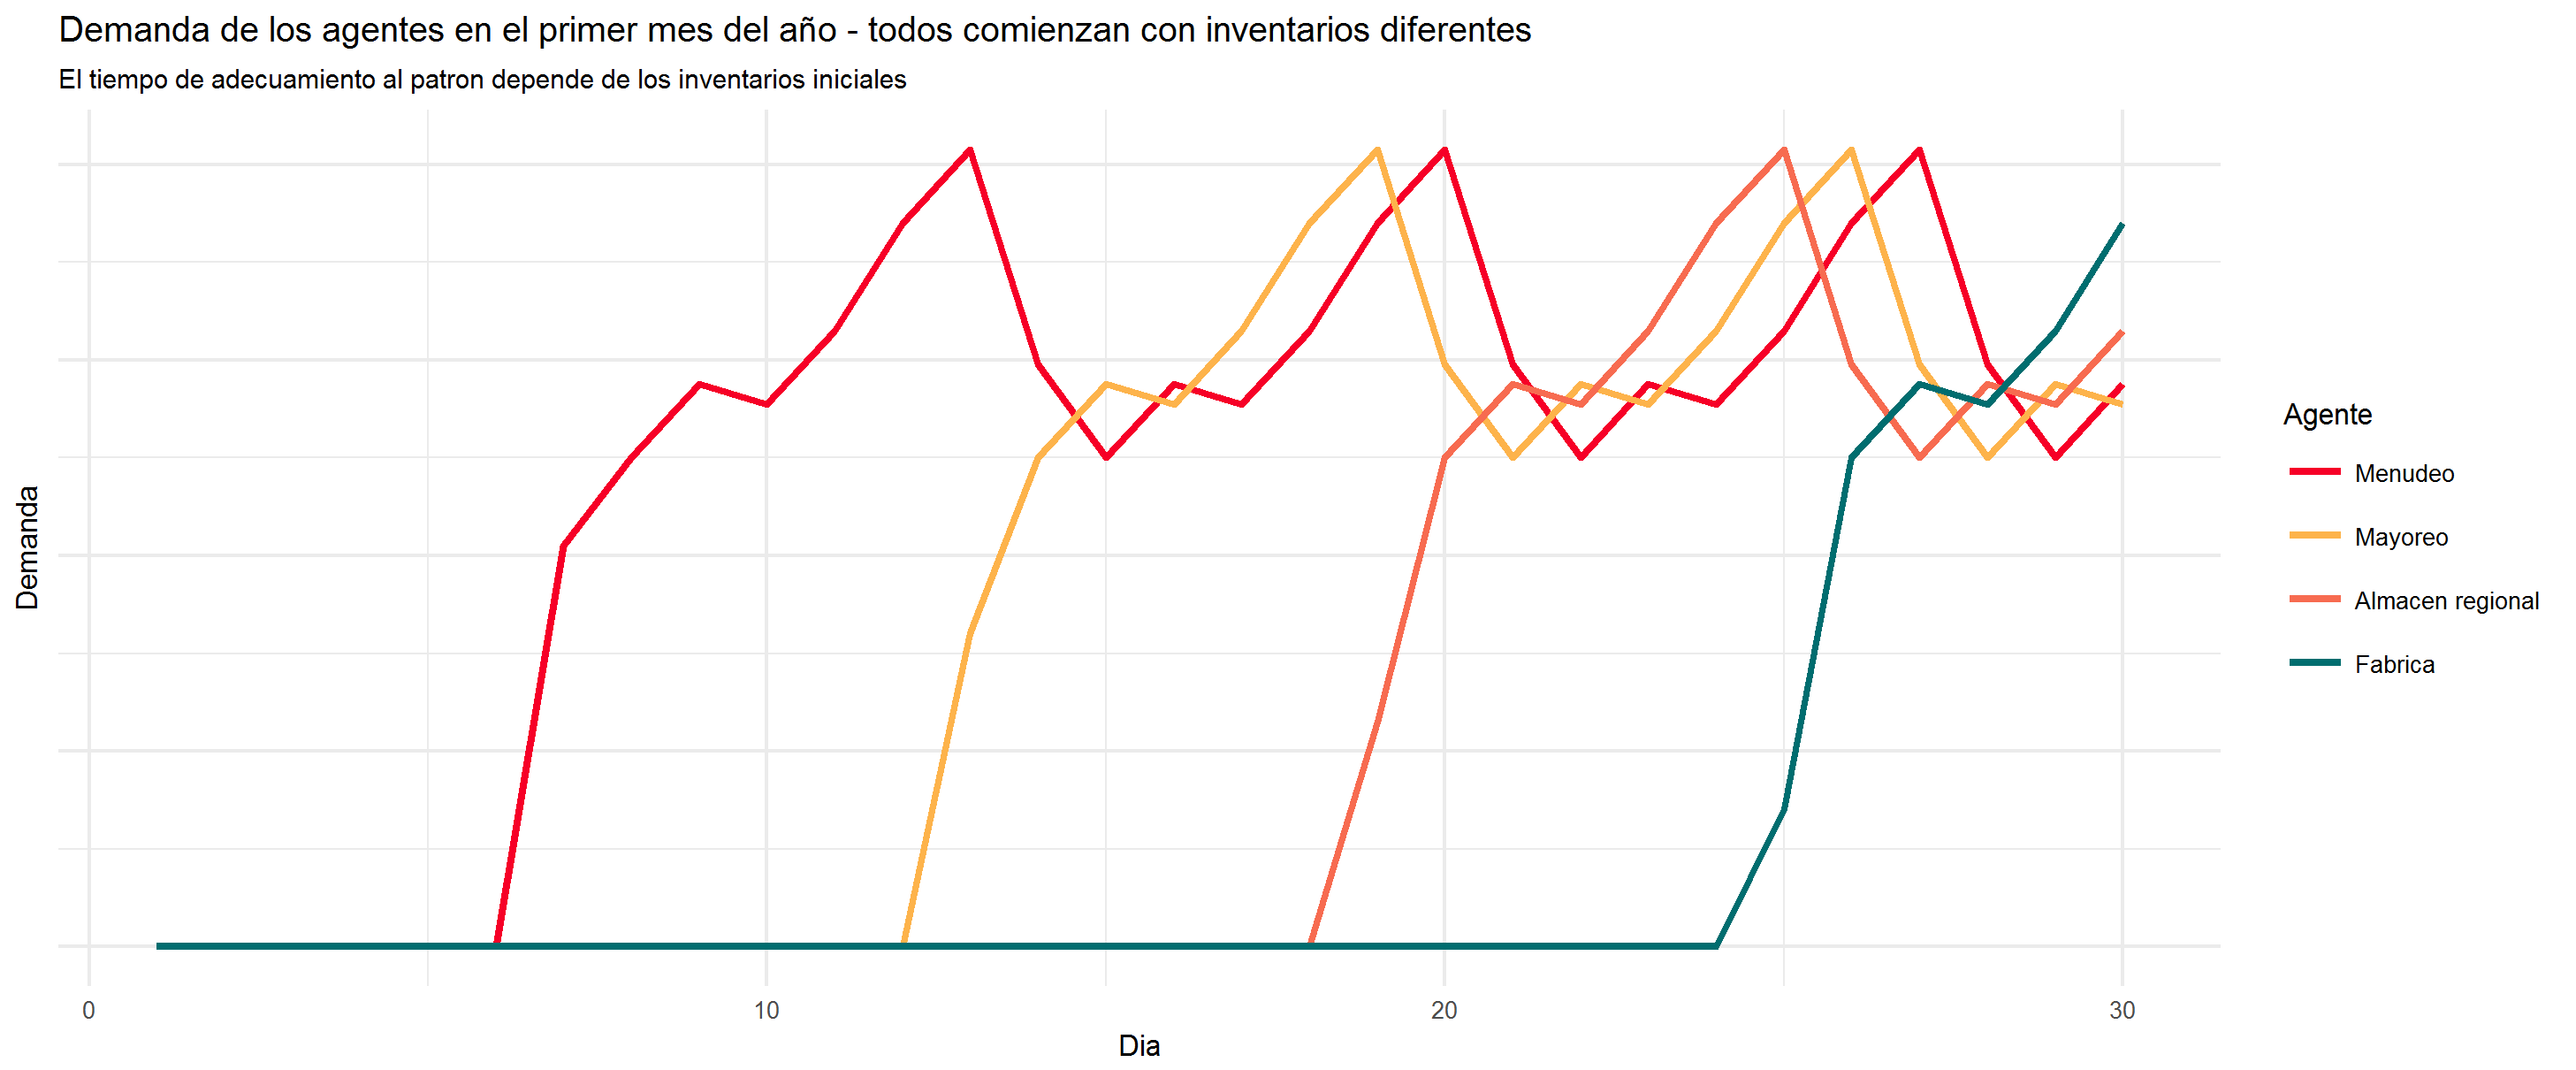
\includegraphics[width=12cm]{tesis_tex/figs/analytic_solution_0_all_45_inv.png}
\centering
\end{figure}

Si la f\'abrica quisiera estimar su demanda para el siguiente a\~no solamente con esta informaci\'on, tendr\'ia que crear un modelo (aunque fuera muy sencillo) para interpolar aquellos d\'ias en los cuales no tuvo informaci\'on. En el caso optimista, usar\'a el mismo patr\'on observado retroactivamente, y tendr\'a una aproximaci\'on relativamente buena. En el caso pesimista, supondr\'a que la demanda del consumidor durante esos d\'ias fue efectivamente cero, y sin duda causar\'a una burbuja de falta de inventario que se propagar\'a hacia abajo en la cadena de suministro. El efecto l\'atigo habr\'a hecho de las suyas.\\

\section{Estacional y aleatoria: m\'as parecido al mundo real}

En el mundo real, ning\'un producto tiene una demanda perfectamente constante. M\'as a\'un, existen una infinidad de productos cuya demanda var\'ia con un patr\'on estacional: por ejemplo, las medicinas antigripales se venden m\'as en invierno. La cerveza (y, en general, las bebidas alcoh\'olicas) tambi\'en siguen este tipo de patrones.\\

En primer lugar, existe un patr\'on semanal bastante esperado: seg\'un \citet{gallupbeer}, se consume m\'as cerveza los fines de semana (ver la figura \ref{weekly_base}). Adem\'as, existe un patr\'on relacionado a las festividades comunes: por ejemplo, en EUA el consumo de bebidas alcoh\'olicas se duplica en las festividades navide\~nas. \\

\begin{figure}[ht!]
\caption{Ejemplo de un Mes T\'ipico}
\label{weekly_base}
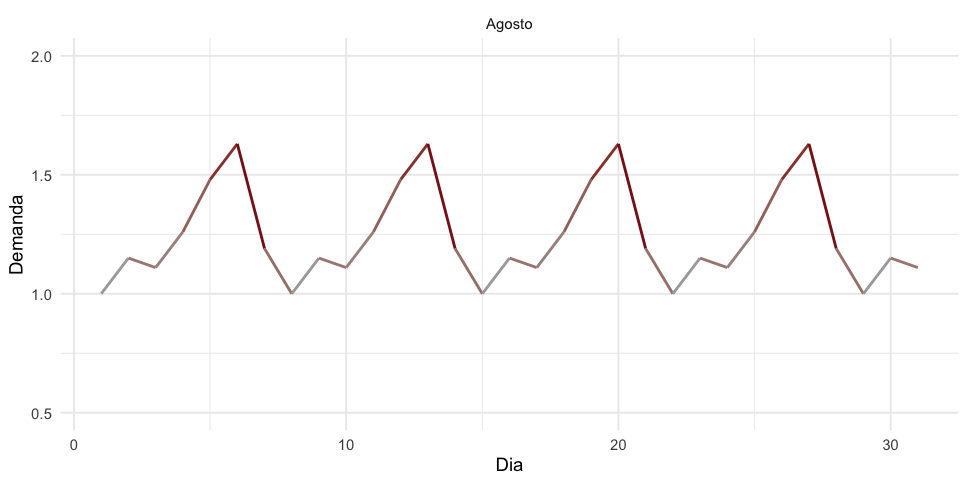
\includegraphics[width=12cm]{tesis_tex/figs/monthly_customer_demand_ggplot.png}
\centering
\end{figure}

Para el presente trabajo, se combinar\'an los dos patrones descritos anteriormente, y se a\~nadir\'a un peque\~no componente aleatorio que cambiar\'a la demanda cada a\~no. El comportamiento ''base'' de la demanda se puede consultar en la figura \ref{yearly_base}. En ella, se puede vislumbrar el patr\'on de aumento cada fin de semana, as\'i como un incremento en las festividades navide\~nas y un pico creado por la fiesta de Independencia de M\'exico. Un ejemplo del comportamiento base, pero perturbado por un poco de aleatoriedad se puede consultar en la figura \ref{yearly_base_noisy}. Sin embargo, cabe mencionar que este es un modelo simple, pues en algunas regiones, podr\'ia tambi\'en existir un patr\'on relacionado al clima, o incluso un alza en la demanda siguiendo temporadas deportivas. \\

\begin{figure}[ht!]
\caption{Demanda Anual de Cerveza}
\label{yearly_base}
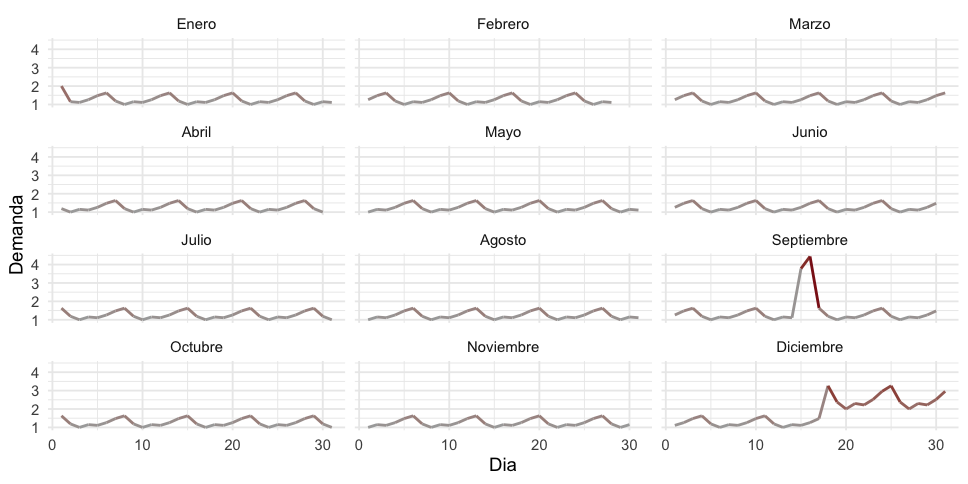
\includegraphics[width=13cm]{tesis_tex/figs/monthly_demand_ggplot.png}
\centering
\end{figure}

\begin{figure}[ht!]
\caption{Realizaci\'on de una Demanda Anual de Cerveza con ruido }
\label{yearly_base_noisy}
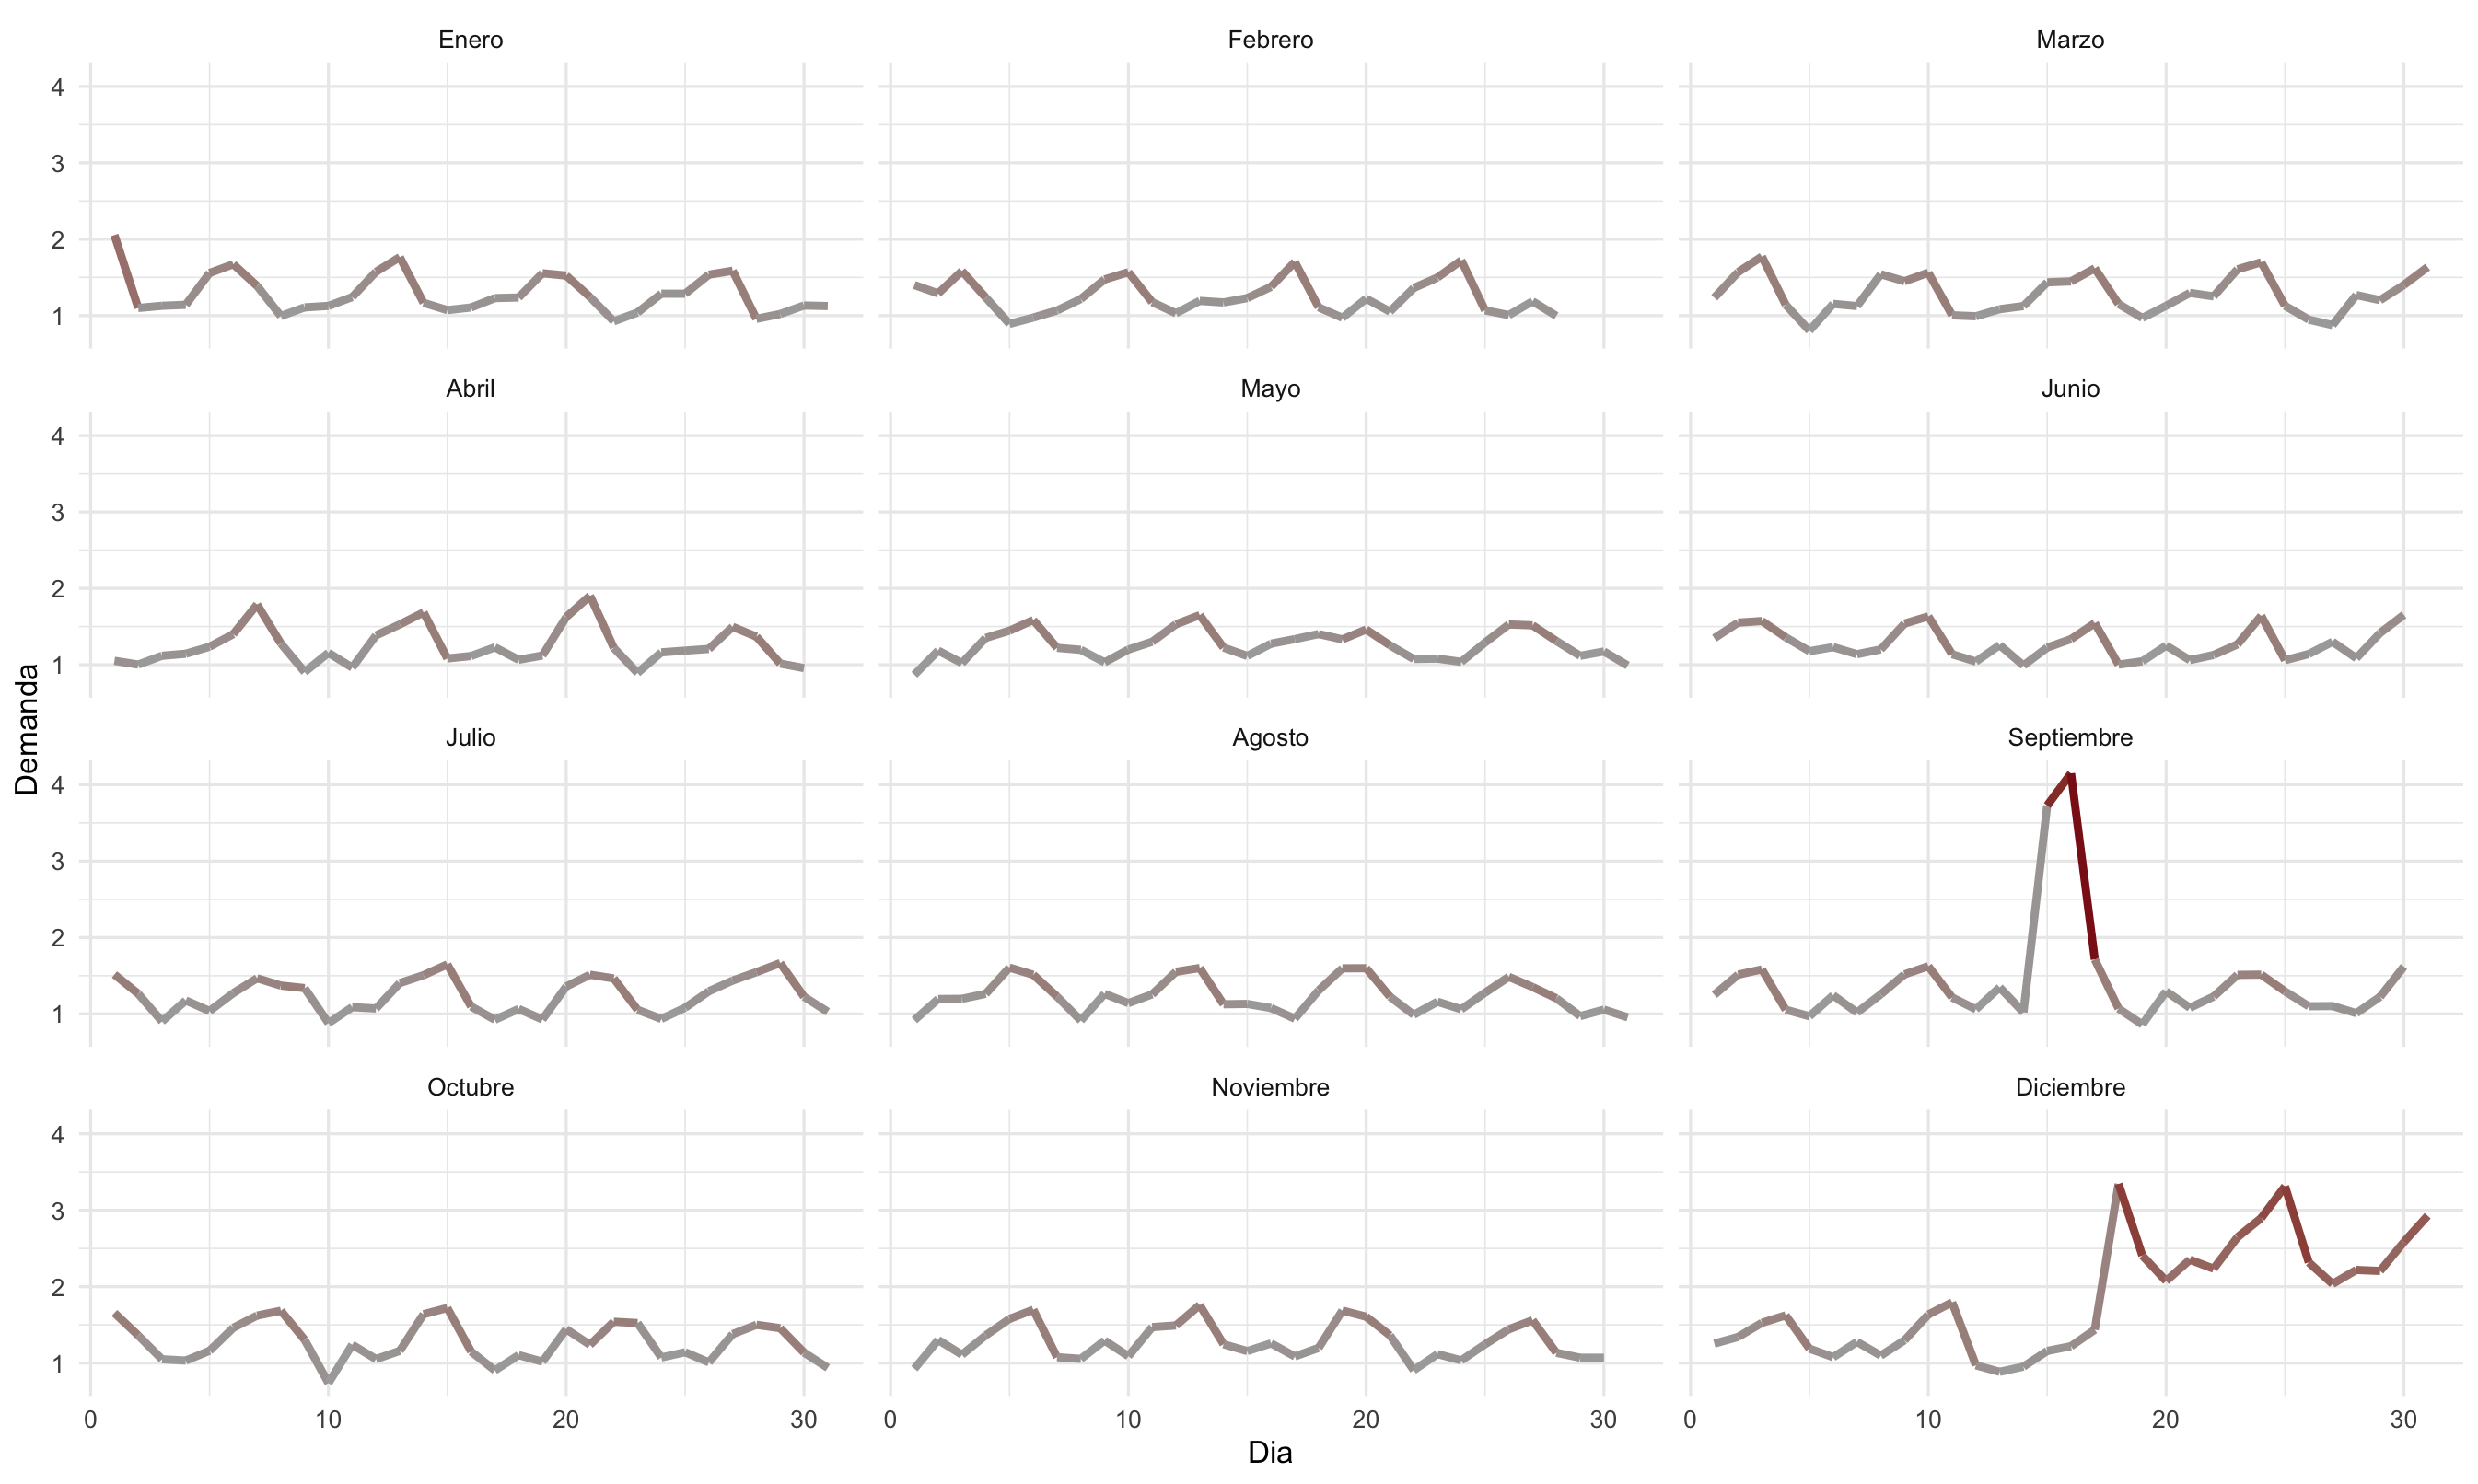
\includegraphics[width=13cm]{tesis_tex/figs/monthly_demand_with_noise_ggplot.png}
\centering
\end{figure}

Como el comportamiento var\'ia a lo largo del a\~no y existe un costo por almacenar inventario, cada agente debe prepararse con adecuada anticipaci\'on para los picos de demanda. Adem\'as, el componente aleatorio resulta en la necesidad de conservar inventario de seguridad (en ingl\'es, \textit{safety stock}) para asegurar que la demanda ser\'a cubierta la mayor parte del tiempo.

\section{Q-Learning}

\citet{Chaharsooghi} public\'o ya un acercamiento a este problema usando \textit{Q-learning}, sin embargo la soluci\'on que encuentra implica que los inventarios (al final del d\'ia, despu\'es de las transacciones del d\'ia) se aproximan a cero, consecuencia directa de que los agentes minimizan su costo de inventario. Adem\'as, la demanda del consumidor obedece a un patr\'on aleatorio.\\

Sin embargo, ninguna de estas soluciones considera dos factores importantes del mundo real: la temporalidad de la demanda (por ejemplo, para la cerveza la cantidad demandada es mayor durante el fin de semana) y la restricción de temporalidad de producci\'on de materias primas. En el mundo agr\'icola, los campos solamente producen ciertas cosechas en ciertos periodos, y es necesario tener suficiente inventario para cubrir la demanda durante todo el a\~no. En el siguiente cap\'itulo, se presentar\'a este escenario como un nivel extra de complejidad al modelo, limitando la oferta de cebada por parte de los campos.
\chapter{La Complicaci\'on: Restricci\'on de Estacionalidad en los Campos}

En su mayor parte, las soluciones al juego de distribuci\'on de cerveza que se han propuesto anteriormente suponen que el agente al final de la cadena (el proveedor de materias primas) tiene inventario infinito. Sin embargo, en la vida real esta situaci\'on no se presenta: especialmente en materias primas que provienen del campo, existen ciclos de siembra y cosecha. Para construir el modelo de la manera m\'as aplicable a la realidad posible, se puede agregar la restricci\'on correspondiente: el productor de materias primas solamente lo hace en ciertos momentos del a\~no.\\

Utilizando los datos m\'as recientes disponibles del departamento de agricultura de los Estados Unidos de Am\'erica (ver \citet{USDA}) se han obtenido los ciclos naturales de uno de los principales componentes de la cerveza, la cebada, los cuales se pueden consultar en la figura \ref{fields}. Es posible observar que la producci\'on es nula entre octubre y mayo, con la mayor parte concentrada en agosto y comienzos de septiembre. Dependiendo de la magnitud de la demanda comparada con la oferta, esto podr\'ia significar que la cadena de suministro tiene que surtirse de cebada durante este periodo para poder cubrir la demanda del resto del a\~no, haciendo uso de la capacidad de almacenamiento en sus respectivos almacenes.\\

\begin{figure}[ht!]
\caption{ }
\label{fields}
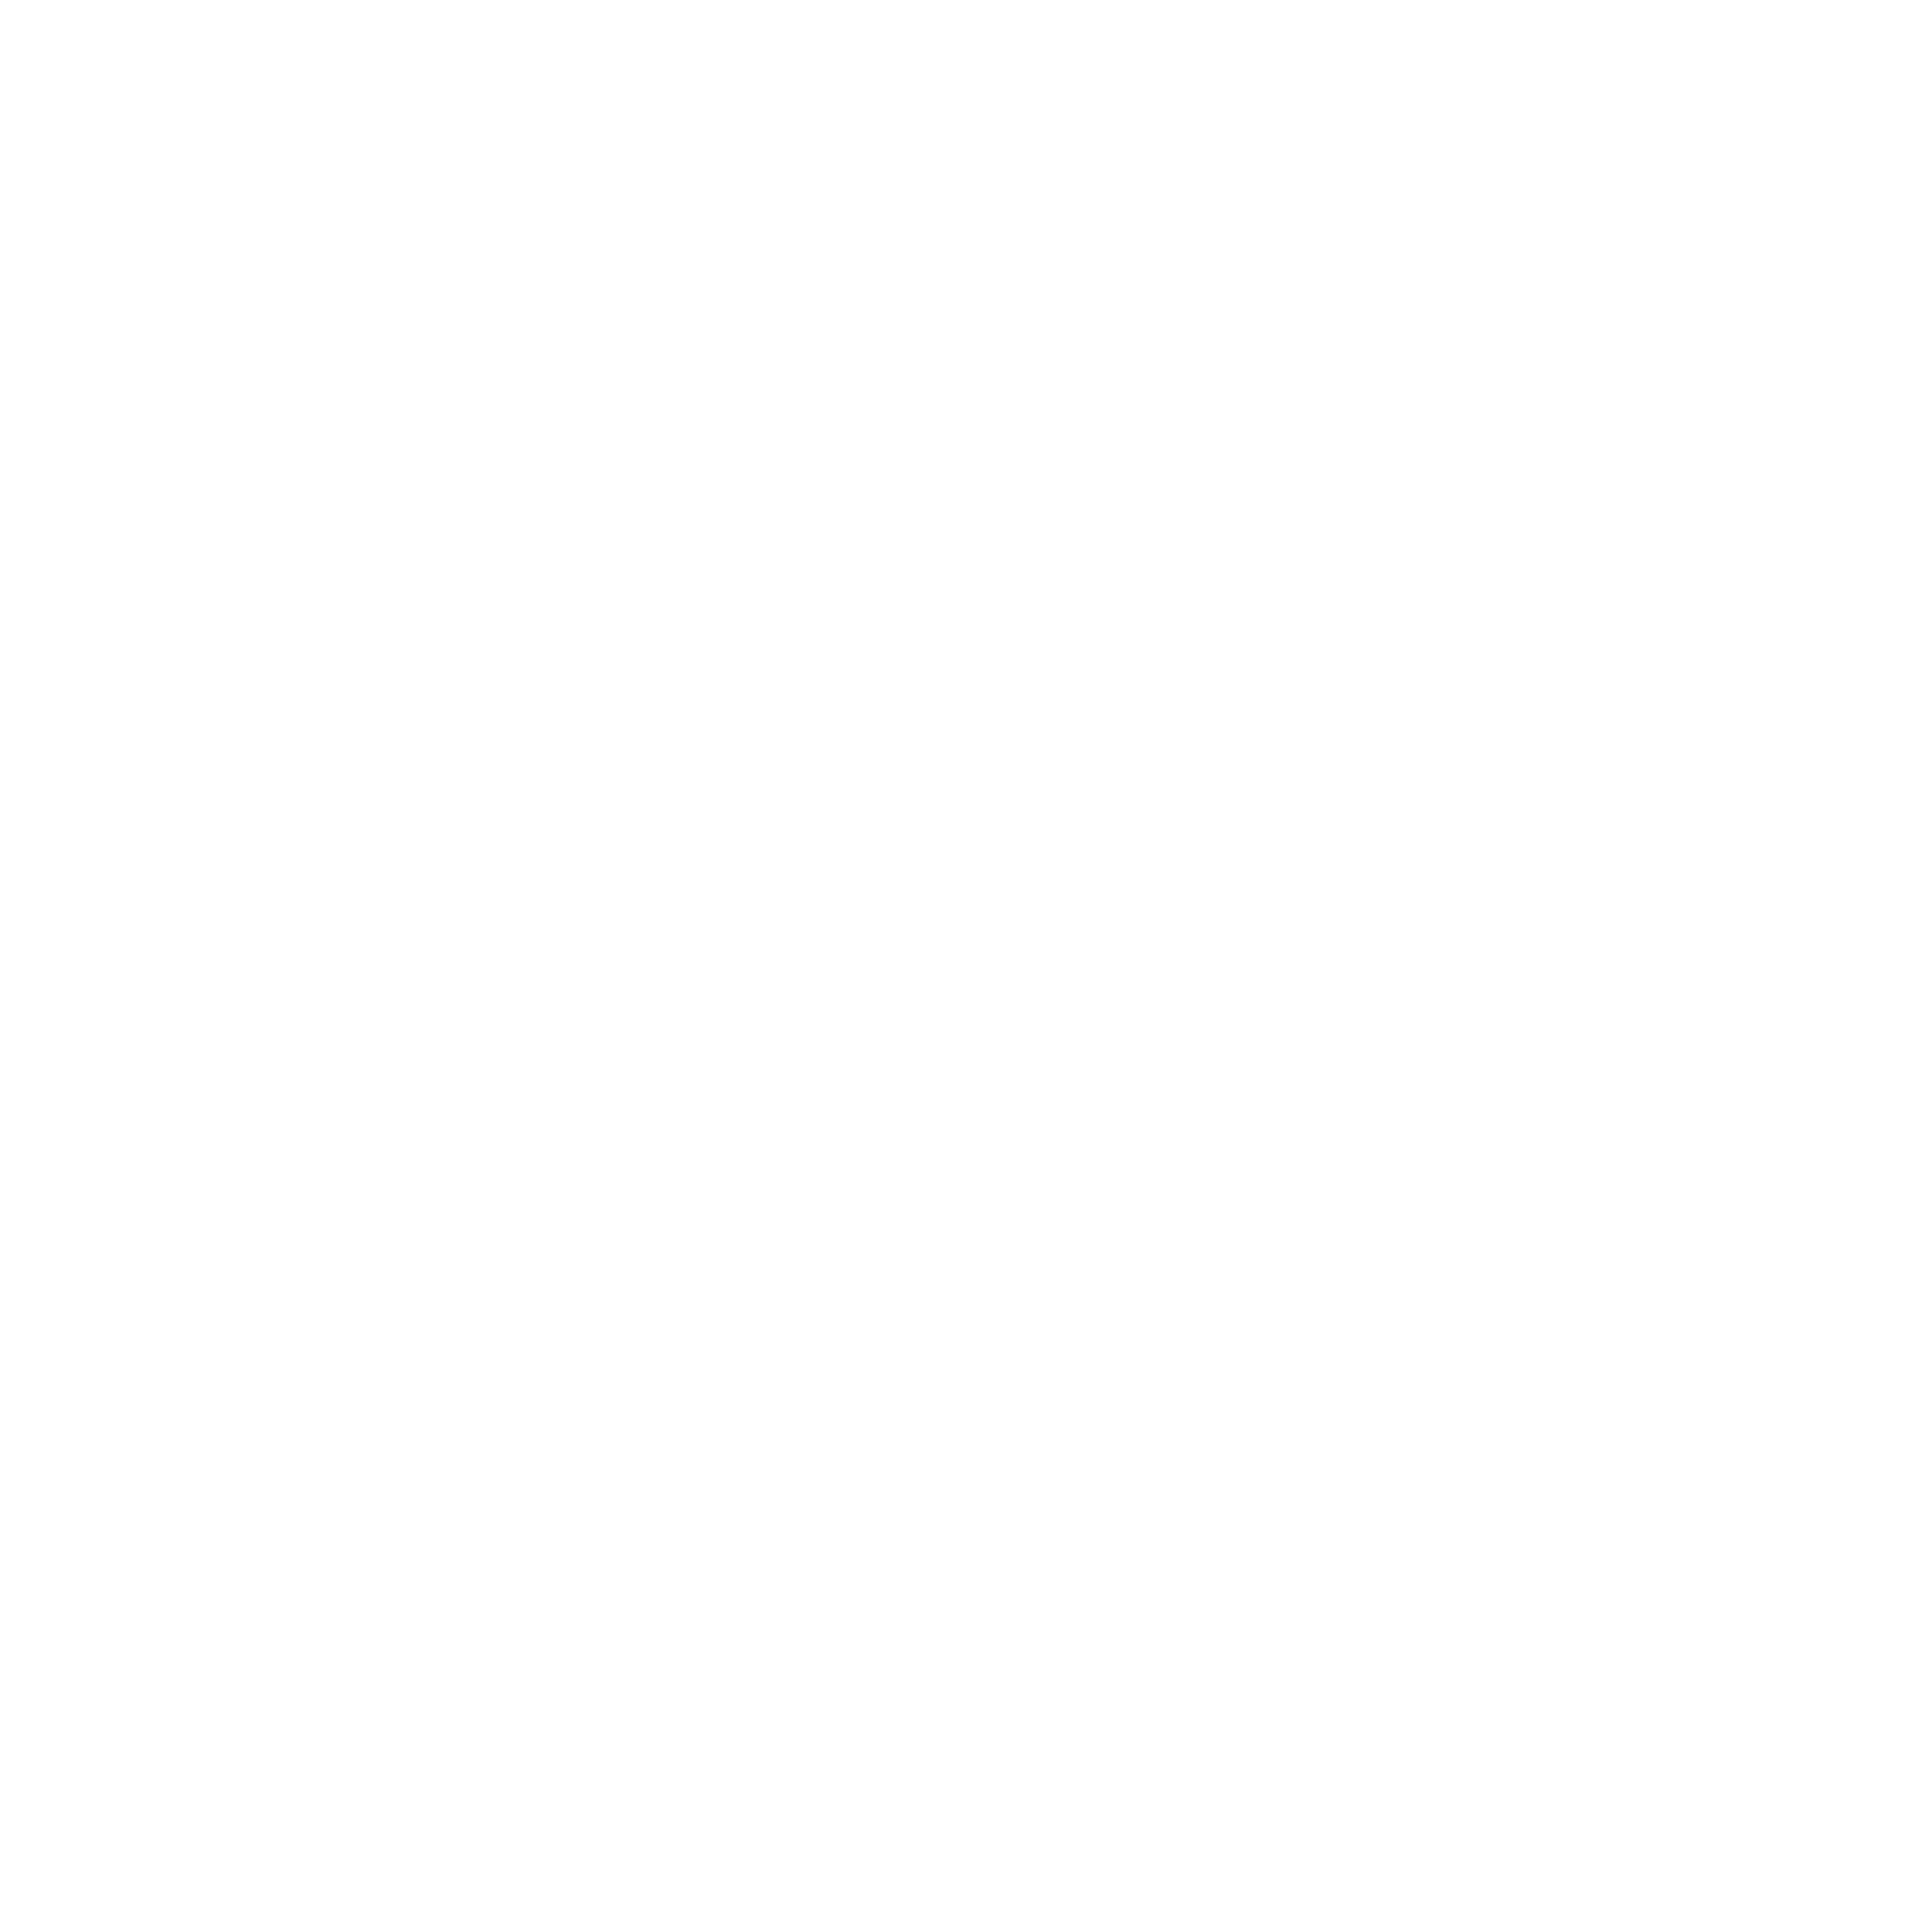
\includegraphics[width=13cm]{fields_monthly_supply_ggplot.png}
\centering
\end{figure}

En la figura \ref{analytic_3} se puede ver el comportamiento de la demanda del consumidor(el cual fue descrito en cap\'itulos anteriores) en rosa; el de la producci'on en los campos, ahora con restricci\'on, en verde; y la demanda de cada agente, en negro. \\

Si todos los agentes tomaran las decisiones relacionadas a la simple m\'axima ``pide hoy lo que esperas vender ma\~nana'', entonces el resultado estar\'ia lejos de ser el \'optimo.
En este escenario se presentan varios efectos: 
\begin{itemize}
    \item Cada agente cuenta con inventario inicial, as\'i que tarda en comenzar a hacer pedidos al agente inmediatamente superior
    \item Cada agente deja de pedirle al agente inmediatamente superior cuando el segundo ya no tiene inventario. Esto es especialmente notorio para la f\'abrica: comienza a tener demanda positiva cuando ya hay producci\'on en los campos, cerca del d\'ia 150
    \item Si la oferta es m\'as baja que la demanda, los agentes piden todo lo que haya disponible, pues es preferible cubrir la demanda parcialmente que no cubrirla en lo absoluto
    \item Los agentes se preparan adecuadamente para el pico de septiembre, con un poco m\'as de anticipaci\'on a medida que se encuentran m\'as lejos del consumidor
    \item Sin embargo, ninguno de los agentes aprende que deber\'ia comprar mucho m\'as en el periodo de producci\'on de los campos (en verde) para poder cubrir la demanda de todo el a\~no (en rosa) y maximizar su ganancia
\end{itemize}

\begin{figure}[ht!]
\caption{Demanda de cada agente durante el a\~no, suponiendo falta de almacenes}
\label{analytic_3}
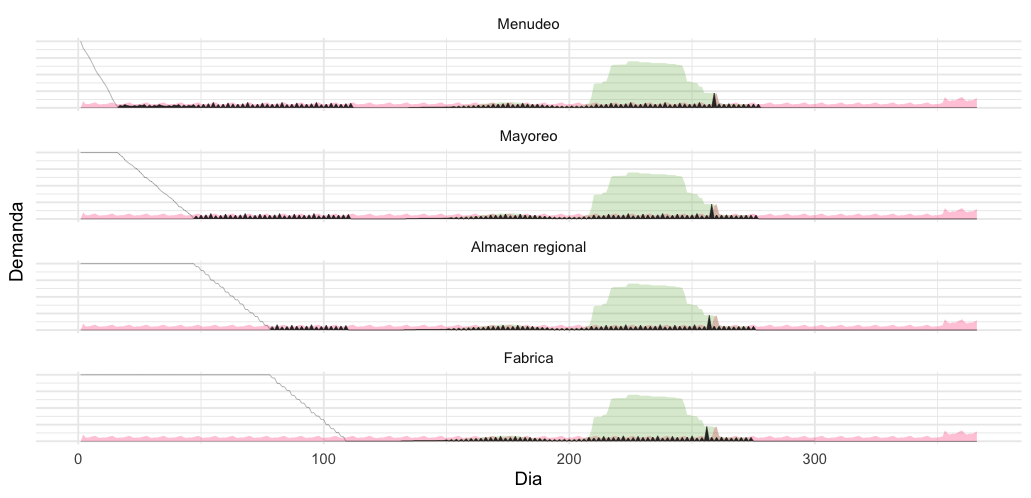
\includegraphics[width=16cm]{tesis_tex/figs/analytic_with_fields_restriction.png}
\centering
\end{figure}

Como se puede observar en la figura \ref{analytic_3}, los agentes no se prepararon adecuadamente para cubrir la demanda posterior al tiempo en que los campos tuvieron producci\'on positiva. Esto sucede porque, en este modelo, los agentes ven solamente un periodo hacia el futuro, as\'i que solo se preparan para ese d\'ia. Esta complicaci\'on vuelve imperante que todos los agentes usen sus almacenes para poder afrontar la demanda, incluso cuando no hay producci\'on. Tal soluci\'on se vuelve compleja porque hay muchos par\'ametros en juego, por mencionar algunos:
\begin{itemize}
    \item El costo diario de almacenamiento influye directamente en qu\'e tanto tiempo un agente puede mantener la cerveza en inventario para cubrir una venta futura, tal que a\'un obtenga un margen positivo cuando \'esta suceda. Si es relevante asegurar que nunca tendr\'an cerveza guardada durante m\'as de un a\~no, o durante cualquier periodo relacionado, por ejemplo, con la caducidad del producto, es necesario que se cumpla la restricci\'on:
    $$
    margen_{agente} <= 365*almacenaje_{agente}
    $$
    \item El castigo por orden no cumplida (\textit{metapolicy}) tambi\'en juega un papel importante en la interacci\'on anterior: si es suficientemente grande, incluso podr\'ia resultar en que un margen negativo causado por el costo de almacenamiento es a\'un preferible a las consecuencias de perder la venta. Si se busca asegurar que siempre sea preferible buscar una venta, es necesario que se cumpla la restricci\'on:
    $$
    castigo_{agente} >= margen_{agente} + 365*almacenaje_{agente}
    $$
    \item Si la producci\'on total en el a\~no es mayor que la demanda total durante el mismo periodo, no es necesario comprarle toda la cebada a los campos. Paralelamente, si la producci\'on es menor a la demanda, es necesario comprar toda la cebada disponible, pues completar algunas ventas siempre es preferible a no completar ninguna
\end{itemize}

Sin embargo, algunas de estas condiciones son te\'oricas y no forzosamente deben cumplirse: es posible que mantener una cerveza en el inventario desde finales de septiembre hasta principios de mayo (cuando vuelve a haber producci\'on) sencillamente no sea redituable. \\

En este trabajo presentaremos un modelo con esta restricci\'on, y lo resolveremos tanto con \textit{policy iteration} como con \textit{Q-learning}. Ambos modelos de aprendizaje reforzado presentados en esta tesis son capaces de capturar todas estas interacciones e incorporarlas al aprendizaje de cada agente.

\chapter{El Producto de Datos}

Se cre\'o un pipeline completo que toma los par\'ametros iniciales, los cuales consisten tanto en condiciones del mundo como en los datos hist\'oricos de demanda y oferta; ejecuta el modelo de aprendizaje elegido (ya sea \textit{policy iteration} o \textit{Q-learning}; y por \'ultimo inserta los resultados en una base de datos para hacer posible consulta y an\'alisis posteriores.\\

\begin{figure}[ht]
\caption{\textit{Pipeline} del proceso}
\label{pipeline}
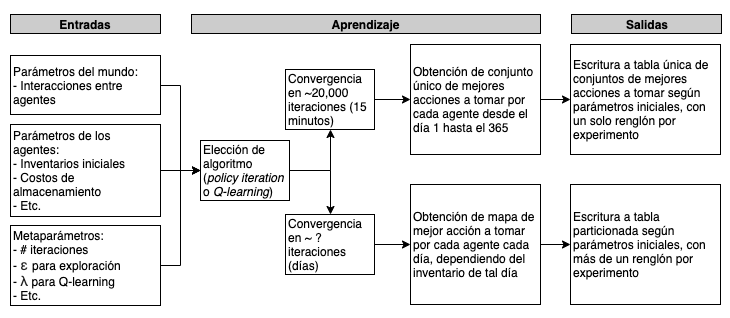
\includegraphics[width=15cm]{pipeline.PNG}
\centering
\end{figure}

Al construir la base en la cual se albergan los resultados, se adoptaron las mejores pr\'acticas para creaci\'on de bases de datos, esquemas y tablas: siguen una estructura espec\'ifica com\'unmente llamada \textit{tidy} (limpia), en la cual cada variable es una columna, cada observaci\'on una fila y cada tipo de unidad observacional es una tabla.\\

Dado que cada uno de los algoritmos de aprendizaje, \textit{policy iteration} y \textit{q-learning}, tiene requerimentos diferentes y la forma en que presenta resultados es distinta, en la base de datos se construyeron dos esquemas respectivamente, cada uno portando el nombre del algoritmo respectivo.

\section{Policy Iteration}

Es necesario crear tablas que contengan los par\'ametros necesarios: una para el mundo (tales como la demanda y oferta), otra para los agentes (tales como precios de venta, inventarios iniciales) y una \'ultima para los experimentos (los hiperpar\'ametros del algoritmo, tales como $\epsilon$ y $\lambda$). Por otro lado, dado que este m\'etodo produce una pol\'itica en forma de vector de tipo num\'erico, la manera \'optima de almacenar los resultados es en una tabla que contenga como llave el identificador (id) del experimento y el agente, y un rengl\'on por resultado.\\ 

Como llave de las tablas, se asigna el identificador (id) del experimento como el \textit{hashlib}\footnote{Las funciones de \textit{hashing} toman datos de tama\~no arbitrario y los mapean a un \textit{hash} de longitud fija.} de la concantenaci\'on de ciertos atributos de este: el sello de tiempo en el cual fue ejecutado y las \textit{policies} \'optimas de cada uno de los agentes. Esto crea un identificador \'unico y tambi\'en permite revisar que ning\'un dato haya sido modificado manualmente, en caso de que tal revisi\'on sea pertinente.\\

Se obtienen un total de 4 tablas que se relacionan de esta manera\footnote{Representaci\'on de los esquemas obtenida directamente del software }:\\

[Aqui falta el diagrama de las tablas en el esquema Policy Iteration]

% https://stackoverflow.com/questions/3223770/tools-to-generate-database-tables-diagram-with-postgresql

% https://stackoverflow.com/questions/3223770/tools-to-generate-database-tables-diagram-with-postgresql


\section{Q-Learning}

El resultado de este algoritmo es una tabla que relaciona a cada par de (estado, acci\'on) con un valor de la funci\'on Q, as\'i que no es pr\'actico utilizar el mismo formato de tabla de resultados que con \textit{policy iteration}, en el cual un rengl\'on contiene un resultado. Se crea entonces una tabla por resultado, y una tabla extra que relaciona el identificador (id) del experimento con el nombre respectivo de la tabla. El resto de la estructura del esquema es parecido al de \textit{policy iteration}, pues tambi\'en existe necesidad de relacionar los par\'ametros de cada experimento con sus resultados.\\

Debido a la estructura de la base, el n\'umero de tablas es variable, y se relacionan de esta manera:\\ 

[Aqui falta el diagrama de las tablas en el esquema Q-learning]

\section{Especificaciones t\'ecnicas}

Para el proceso se utilizaron PostgreSQL 10 y Python 3.6.5 en la distribuci\'on contenida en Anaconda, as\'i como varios paquetes de Python descritos en el archivo de requerimentos del repositorio de Github. Todos los procesos fueron ejecutados en una computadora Macbook con [] GB de RAM y [] procesadores tipo [].

[Datos faltantes]
\chapter{Resultados}

\section{\textit{Policy Iteration}}

Interesante: a veces no converge a m\'aximos globales para todos los jugadores simult\'aneamente

Algo de tiempo de convergencia - cu\'antas iteraciones son necesarias etc tiempo m\'aquina etc


\section{\textit{Q-Learning}}



\chapter{Conclusiones}



\section{Trabajo futuro}



\appendix
%% Cap'itulos incluidos despues del comando \appendix aparecen como ap'endices
%% de la tesis.
\chapter{Ap\'endice}

\section{Escenarios de \textit{policy iteration}}

En este apartado se recopilan escenarios probados para el algoritmo \textit{Policy Iteration}. Tales escenarios constituyen, en su mayor\'ia, cambios en las condiciones iniciales del mundo, para visualizar los efectos en las estrategias aprendidas.\\

El escenario A muestra los resultados al iniciar uno de los agentes, en este caso el almac\'en regional, con un inventario de $500$ unidades, mientras que los dem\'as comienzan con $10$ unidades. Se puede observar que los agentes inferiores al almac\'en reconocen que hay existencias, y entonces su cantidad demandada es mayor a cero hasta el momento en el que el inventario del almac\'en se termina. Por otro lado, ni el almac\'en ni la f\'abrica presentan demanda constantemente positiva al principio del a\~no, pues ellos no pueden tomar decisiones diferentes en ese periodo debido la inyecci\'on de inventario.\\

Para el escenario B, se utiliz\'o una tendencia de producci\'on en los campos diferente de la utilizada en todo el trabajo, para demostrar que los agentes aprender\'an nuevas tendencias en caso de que estas cambien. Los nuevos valores fueron creados manualmente sin ninguna l\'ogica espec\'ifica. Puede notarse que todos los agentes cambian sus pol\'iticas \'optimas para comprar cuando hay producci\'on en los campos. \\

\begin{figure}[H]
\caption{Escenario A}
\label{scen_wholesale_500}
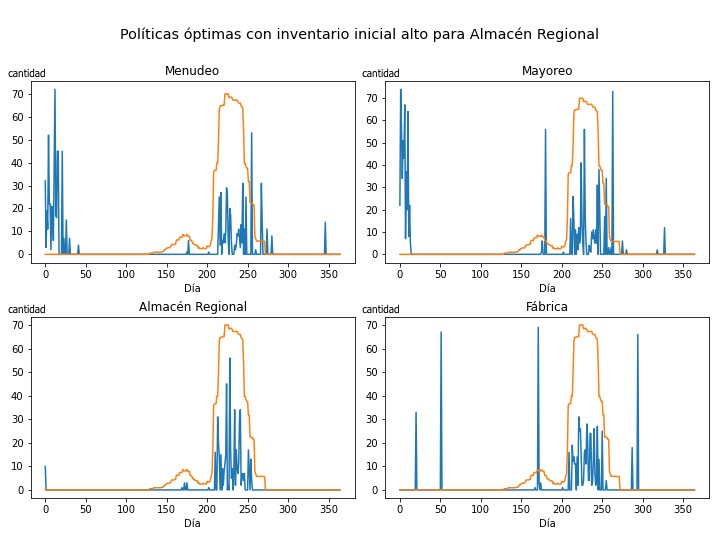
\includegraphics[width=9cm]{tesis_tex/figs/policyiteration_scen_wholesale500.png}
\centering
\end{figure}

\begin{figure}[H]
\caption{Escenario B}
\label{scen_alternative_supply}
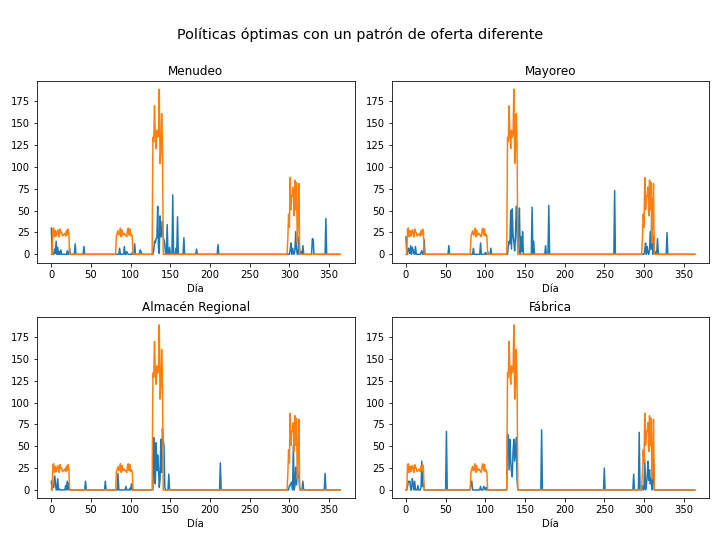
\includegraphics[width=9cm]{tesis_tex/figs/policyiteration_scen_alternativesupply.png}
\centering
\end{figure}
\include{ApendiceB}

%% Incluir la bibliograf'ia. 
\bibliography{Bibliografia}

\end{document}




%%%%%%%%%%%%%%%%%%%%%%%%%% borrar en version final
 % The \cite command functions as follows:
 %   \citet{key} ==>>                Jones et al. (1990)
 %   \citet*{key} ==>>               Jones, Baker, and Smith (1990)
 %   \citep{key} ==>>                (Jones et al., 1990)
 %   \citep*{key} ==>>               (Jones, Baker, and Smith, 1990)
 %   \citep[chap. 2]{key} ==>>       (Jones et al., 1990, chap. 2)
 %   \citep[e.g.][]{key} ==>>        (e.g. Jones et al., 1990)
 %   \citep[e.g.][p. 32]{key} ==>>   (e.g. Jones et al., p. 32)
 %   \citeauthor{key} ==>>           Jones et al.
 %   \citeauthor*{key} ==>>          Jones, Baker, and Smith
 %   \citeyear{key} ==>>             1990
 %---------------------------------------------------------------------
% 
% \begin{center}
%\includegraphics[scale=0.5]{REER1970_Niveles.jpeg}
%\end{center}
% 
% 
% 